\documentclass{article}

\setlength{\parindent}{0pt}

\usepackage{fullpage}
\usepackage{graphicx}

\def\Nat{{\rm I\kern-.17em N}}
\def\SFF{\hbox{I\kern-.09em\hbox{I}}}
\newcommand\Bezier{B\'{e}zier }

\newcommand\projecttitle{OpenGL Jumper}
\newcommand\myname{Ramanpreet Nara}
\newcommand\myuserid{20517713}
\newcommand\mystudentid{rsnara}

\begin{document}

\begin{minipage}[t]{3in}
{\huge \bf
	\projecttitle
}

\medskip
Name: \myname \\
User ID: \myuserid \\
Student ID: \mystudentid
\end{minipage}
\hfill
\begin{minipage}[t]{3in}
%%%% Use the first of these if your image is wider than tall; use the
%%%% second if your image is taller than it is wide.
\vspace{0pt}
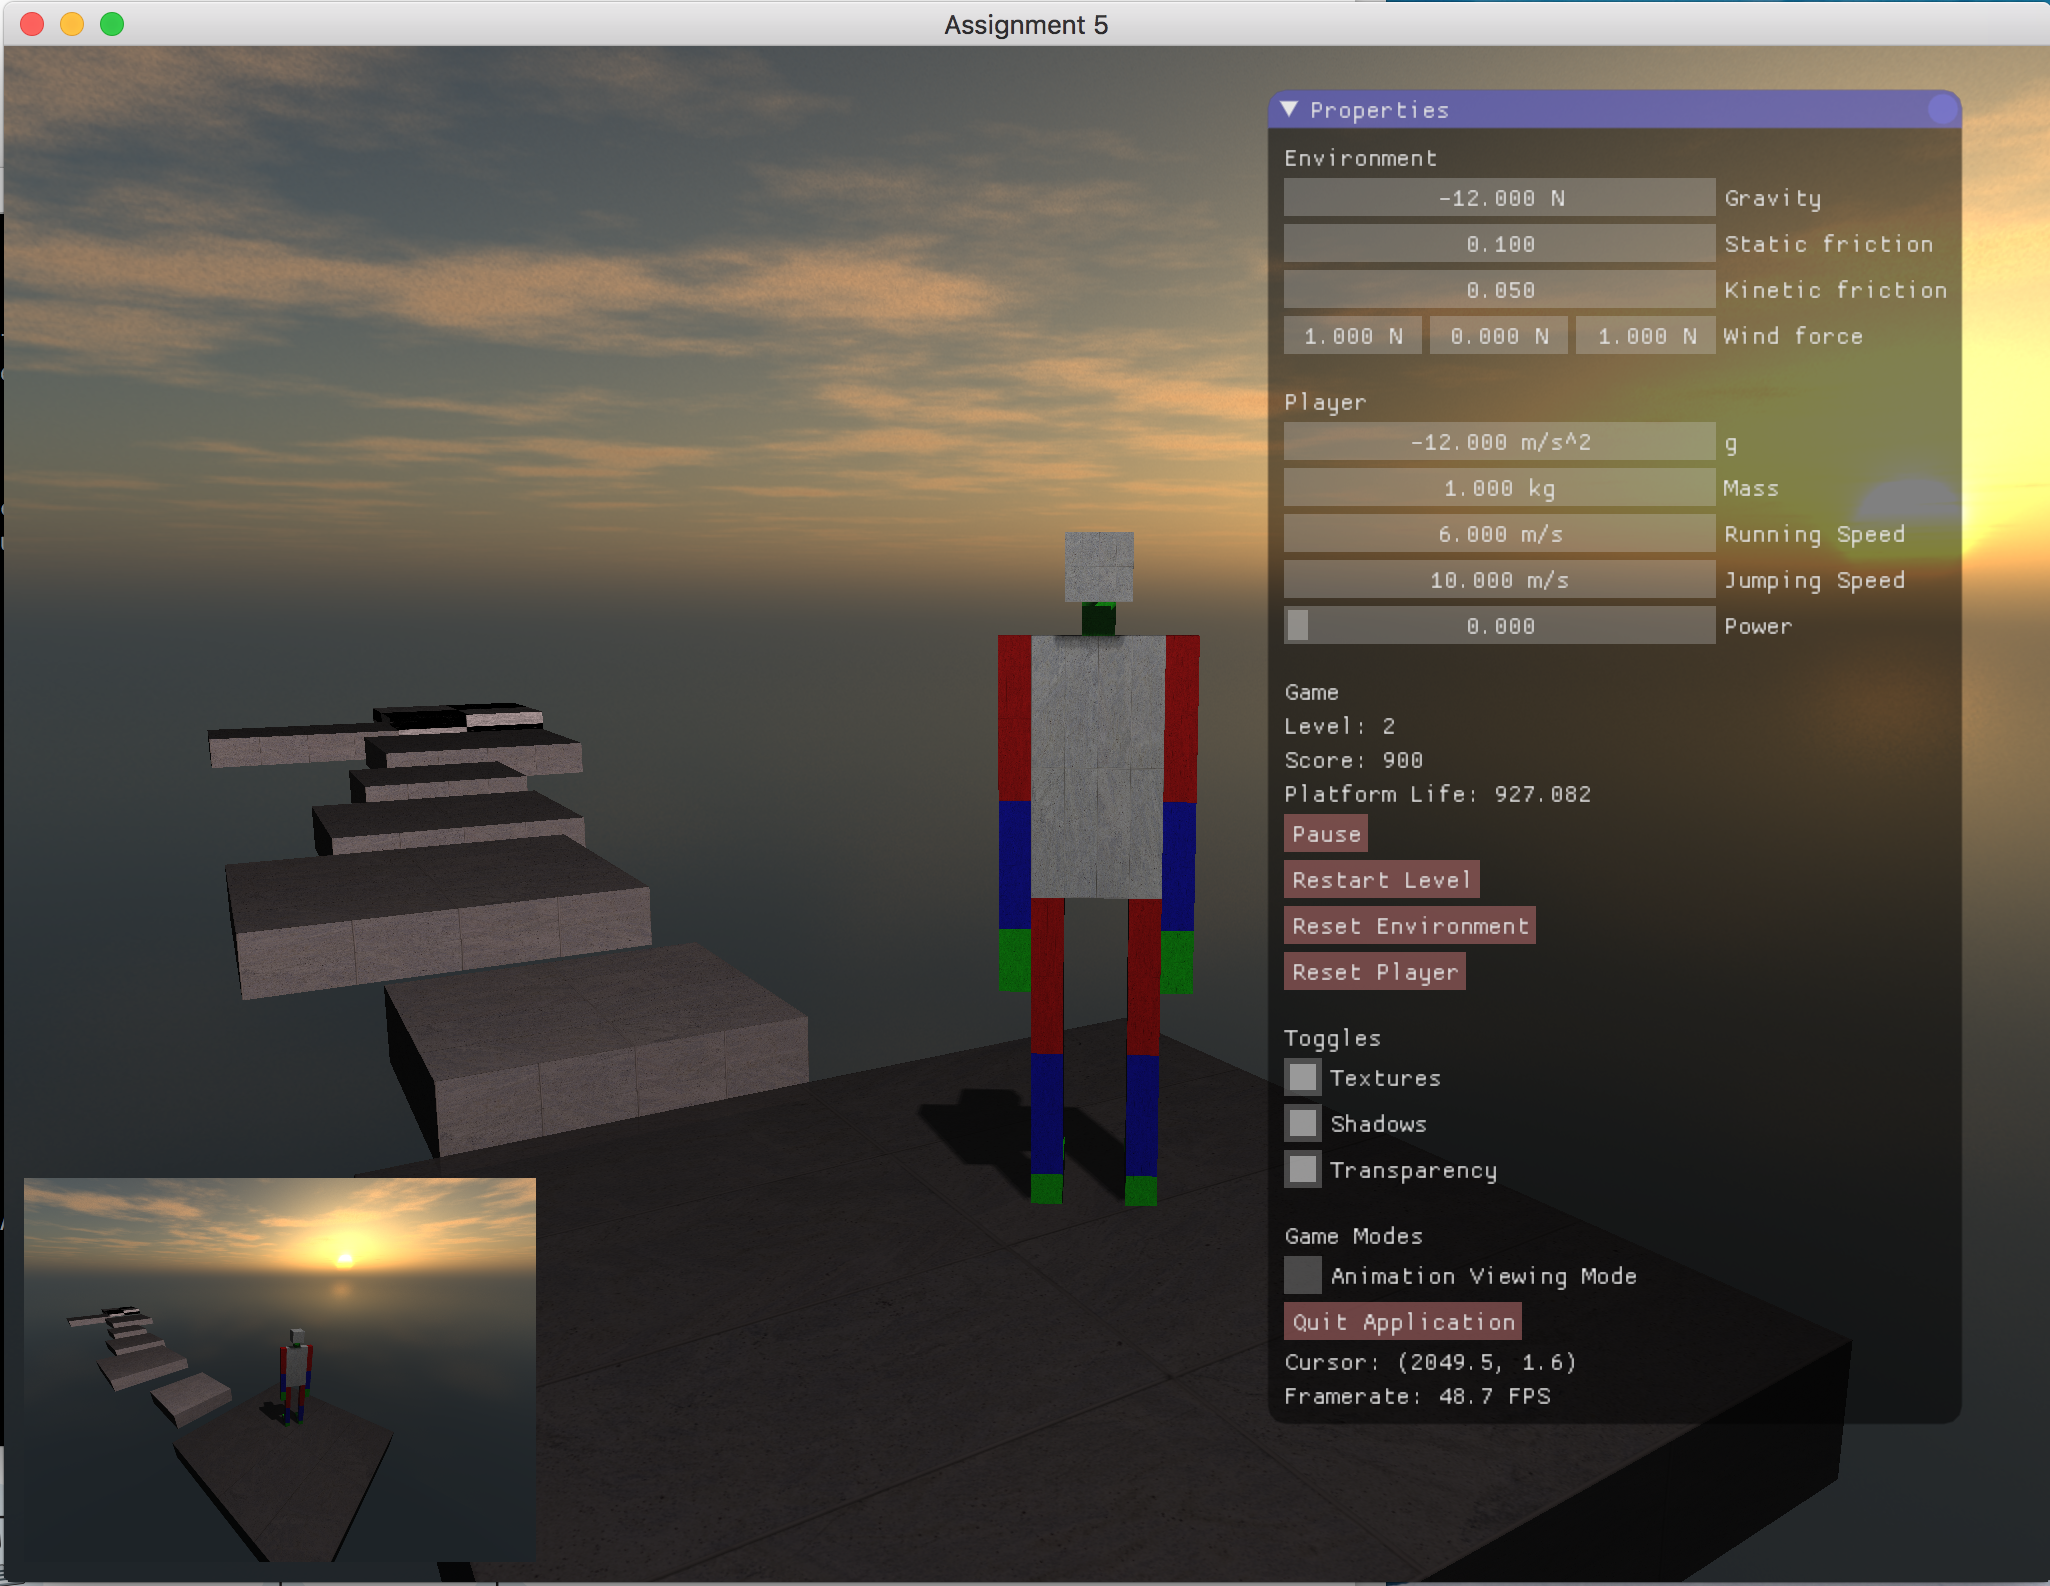
\includegraphics[width=3in]{screenshot.png}   %%%% Change file.png to your image
% \includegraphics[height=2in]{image2-FRONT.png}   %%%% Change file.png to your image
\end{minipage}


\subsection*{Artistic Merit (Polish/Artistry/Humour)}
\vfill
\subsection*{Technical Merit (Algorithms/User Interface/Graphics Techniques)}
\vfill
\subsection*{Difficulty}
\vfill
\subsection*{Code/Documentation/Demo}
\vfill
\subsection*{Mark}
\begin{center}
\begin{tabular}{lr}
Objective Mark: &~~/10\\
Subjective Mark: &~~/6\\
\hline
Total &~~/16
\end{tabular}
\end{center}

\newpage

{\huge \bf
	\projecttitle
}

\medskip
Name: \myname \\
User ID: \myuserid \\
Student ID: \mystudentid

\bigskip
{\Large Objectives}

\hrule
\begin{description}
        \item[\_\_\_ 1:]
          \textbf{Modeling the Scene.} - World objects are rendered on to the screen correctly.

        \item[\_\_\_ 2:]
		  \textbf{UI.} - The mouse and keyboard can be used by the player to control the game objects and camera. A GUI also exists for controlling game settings.


        \item[\_\_\_ 3:]
		  \textbf{Texture mapping.} - It is evident that texture mapping has been employed at least once.


        \item[\_\_\_ 4:]
		  \textbf{Keyframe Animation.} - When the player walks, the puppet plays a walking animation. The current frame is interpolated from its surrounding frames using linear interpolation.


        \item[\_\_\_ 5:]
		  \textbf{Static collisions.} - On each stationary platform, the puppet does not fall through the platform and die.


        \item[\_\_\_ 6:]
	      \textbf{Dynamic collisions.} - On each moving platform, the puppet does not fall through the platform and die.


        \item[\_\_\_ 7:]
		  \textbf{Synchronized sound.} - When the player interacts with the game by moving the puppet, there is audible feedback.


        \item[\_\_\_ 8:]
		  \textbf{Physics Engine} - The puppet is subject to gravitational forces (parameter: $g$) and wind force (parameter: $F_w$). The puppet is also subject to static friction when it's standing on a platform. The static friction is a function of the puppet's mass (parameter: $M$) and the platform's normal.


        \item[\_\_\_ 9:]
		  \textbf{Transparency} - Transparency will be implemented using the alpha channel. At least one game object is transparent.


        \item[\_\_\_ 10:]
		  \textbf{Shadows} - Shadows are implemented using shadow maps.


\end{description}

\hrule

\end{document}
